\documentclass{beamer}
\renewcommand{\baselinestretch}{1.1}
\usepackage{graphicx}
\usepackage{natbib}
\usepackage{amsmath}
\usepackage{hyperref}
\usepackage{listings} 

\def\labelitemi{--}
\parindent=0pt

\usepackage{xcolor}

\colorlet{codecolor}{black!30}
\newcommand{\codebox}[1]{%
  \colorbox{codecolor}{\ttfamily \detokenize{#1}}%
}

\begin{document}
\bibliographystyle{/Users/Lizzie/Documents/EndnoteRelated/Bibtex/styles/besjournals}
\renewcommand{\refname}{\CHead{}}

{\usebackgroundtemplate{%
  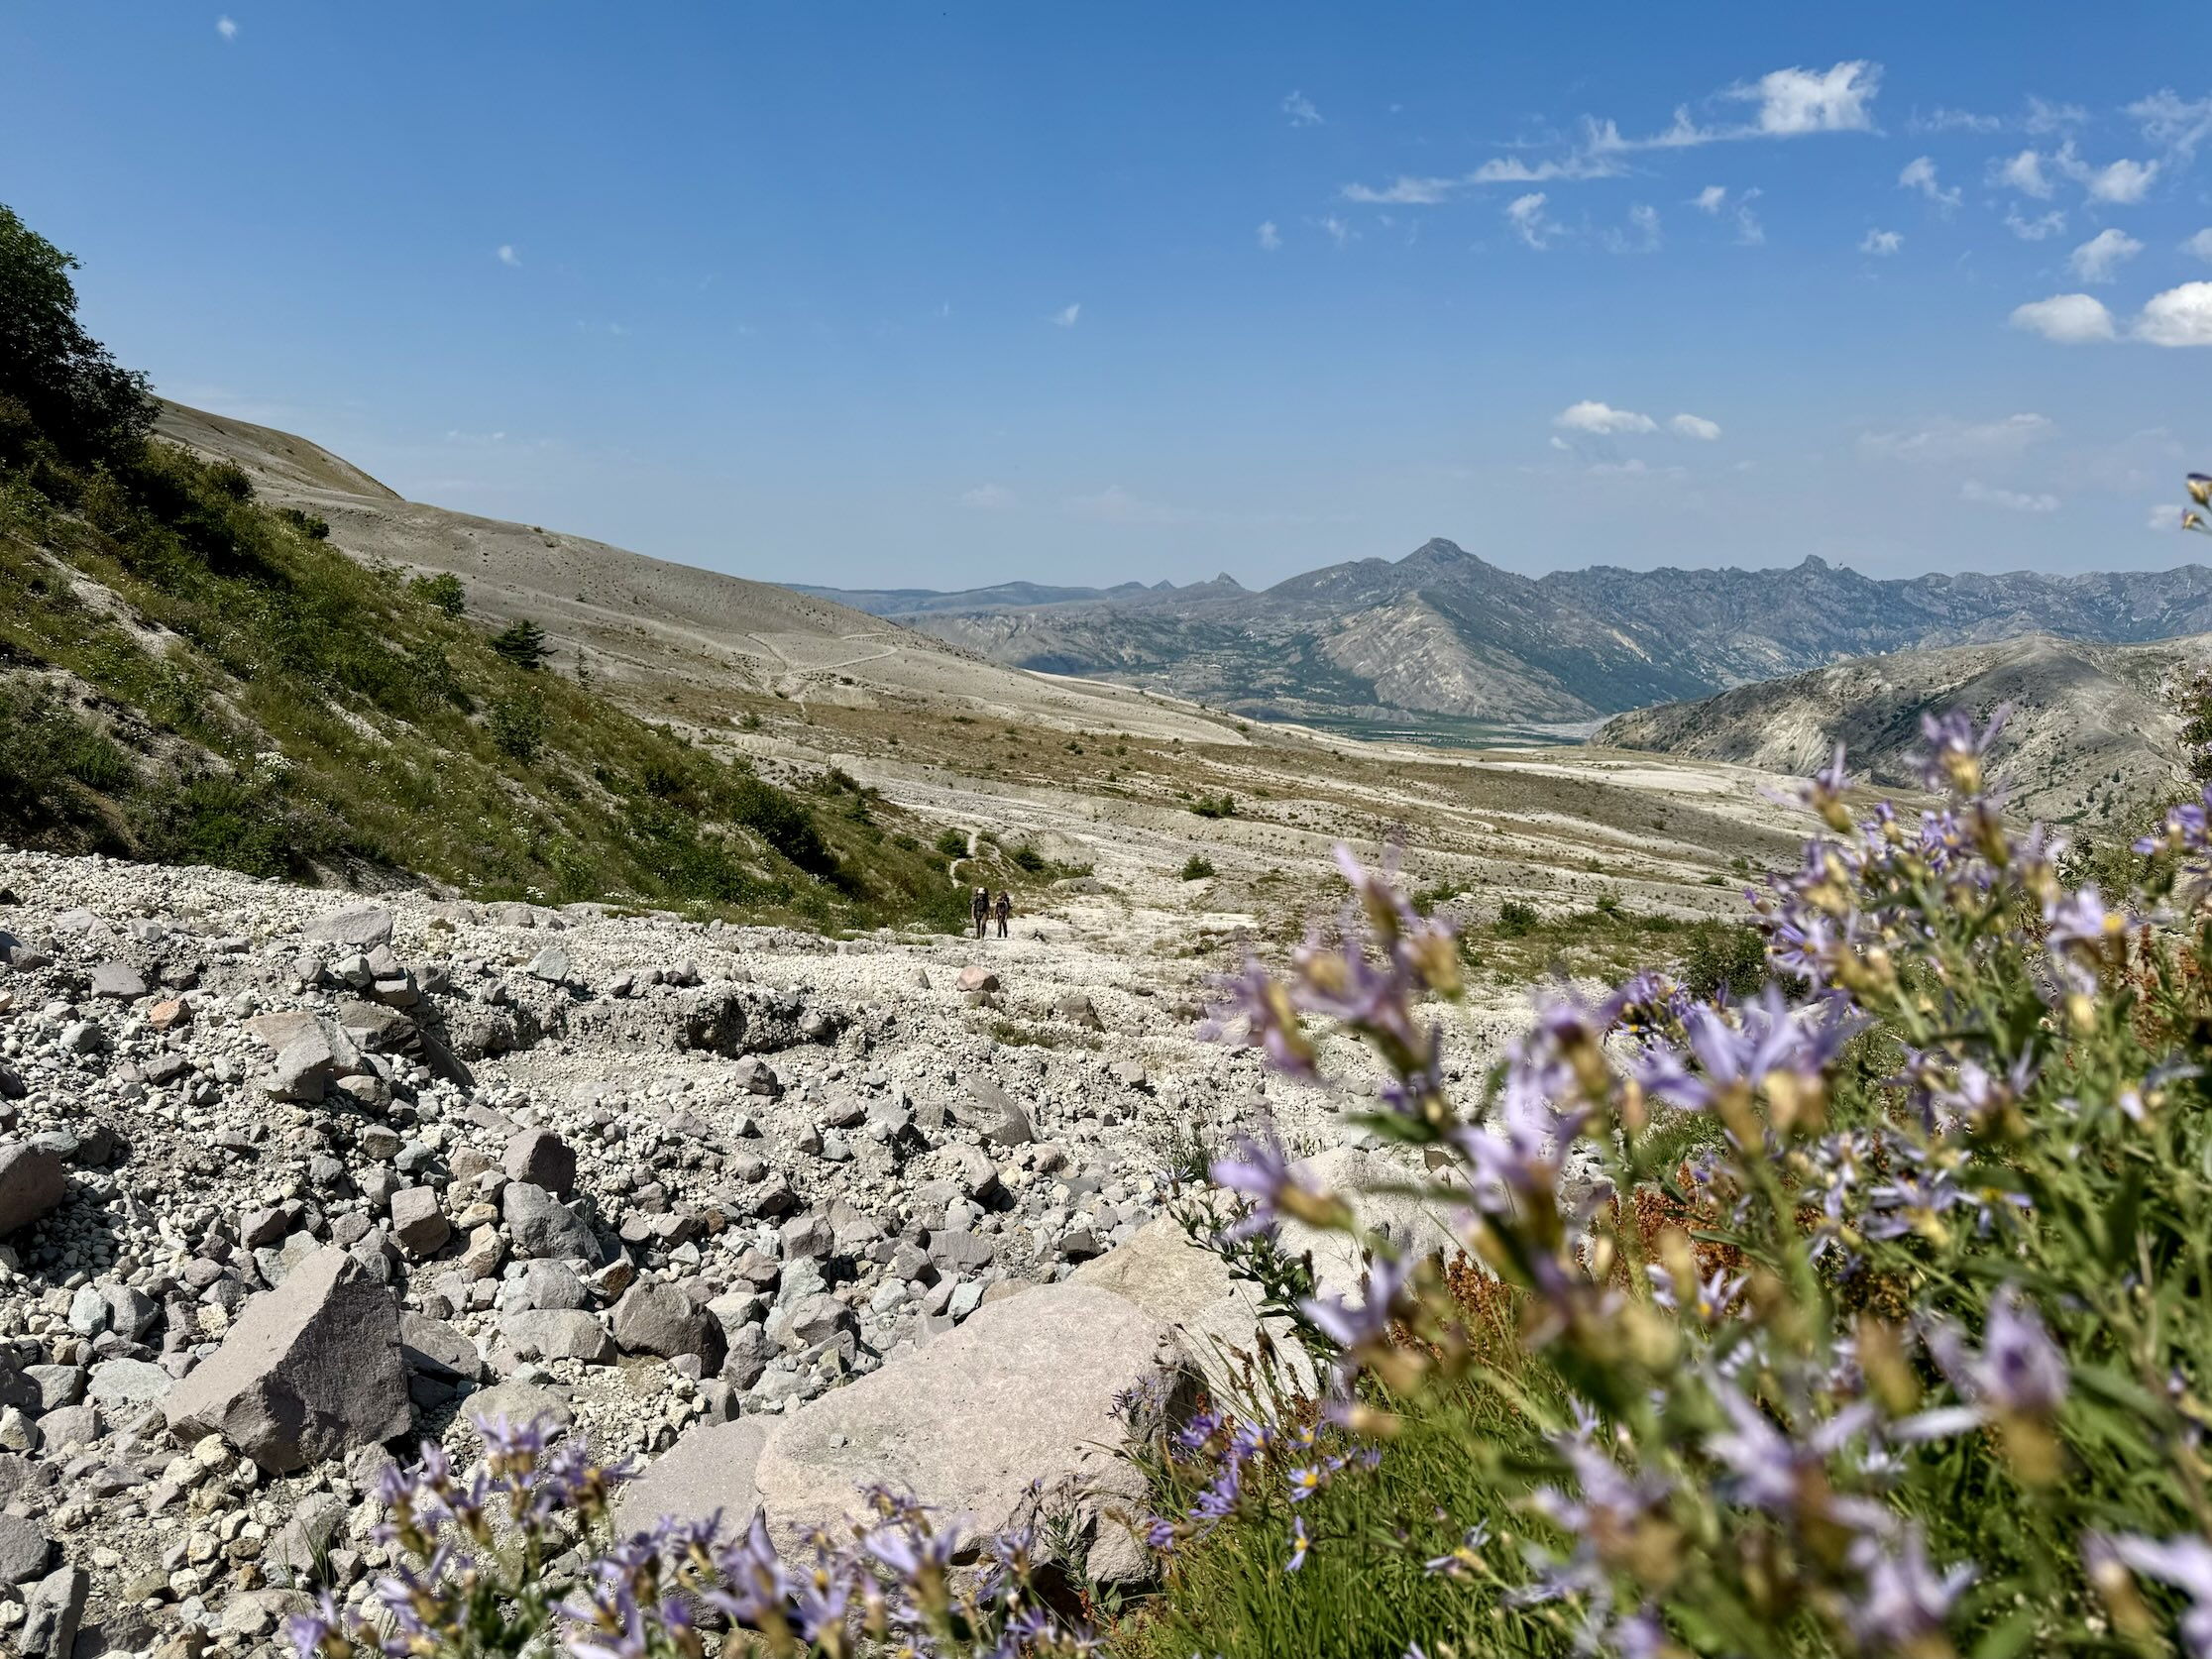
\includegraphics[width=\paperwidth,height=\paperheight]{..//photos/IMG_3133.jpg}} 
\begin{frame}
\begin{center}
\vspace{-20ex}
{\color{white} {\huge Bayesian Model Group}}
\\
\vspace{0ex}
{\color{white} {\Large 5 August 2025}}

\end{center}
\end{frame}
}


	\frame{
		\frametitle{How the group works}
		\framesubtitle{}
		\begin{itemize}
			\item Meets every two weeks with someone presenting their question/model and what they need help on
			\item Learn by ...
				\begin{itemize}
			 	\item Actively helping others with their models
				\item Getting help on your models
				\end{itemize}
		\end{itemize}
	}

	\frame{
		\frametitle{How a group like this succeeds}
		\framesubtitle{}
		\begin{itemize}
			\item Everyone comes every week (within reason) and actively participates
			\item Everyone gives of their time freely in the meetings (no phones, working on other stuff, etc.)
			\item Models are openly shared with data, code etc.
			\item Everyone recognizes that they can help with various aspects of modeling (thinking biologically, coding, etc.)
			\item No model is too simple or complex to present as long as you make it possible for others to follow you! 
		\end{itemize}
	}

	\frame{
		\frametitle{How to present when it's your week}
		\framesubtitle{Some guidelines}
		\begin{itemize}
			\item Clearly state your question and/or aim
			\item Give sufficient background so everyone can engage with the question/aim
			\item Describe where in the workflow you are 
				\begin{itemize}
				\item Formulate model
				\item Simulated data to test model
				\item Fit model to empirical data
				\item Retrodictive checks 
				\end{itemize}
			\item Describe what you need to help with (e.g., formulating the model? Thinking about priors? Developing a retrodictive check?)  
			\item Plan to present for no more than 30 minutes (maximum; we aim for a 60 minute meeting with the room reserved for 90 mins)
		\end{itemize}
	}
	
		\frame{
		\frametitle{How to present when it's your week}
		\framesubtitle{Some more guidelines}
		\begin{itemize}
			\item You can present your model progress multiple times! (\emph{This is how it has worked in the past.})
			\item Share code/data/slides via a public repo or on the meeting repo (slides, code, working from the board are all good ways to present)
			\item I pulled some random examples {\color{orange}\href{https://github.com/temporalecologylab/bayesforeverornot/wiki}{here}}
		\end{itemize}
	}

	\frame{
		\frametitle{Questions \& Scheduling ...}
		\framesubtitle{}
		\begin{itemize}
			\item Questions? 
			\item  {\color{orange}\href{https://github.com/temporalecologylab/bayesforeverornot/wiki}{Sign up!}}
		\end{itemize}
	}


{\usebackgroundtemplate{
  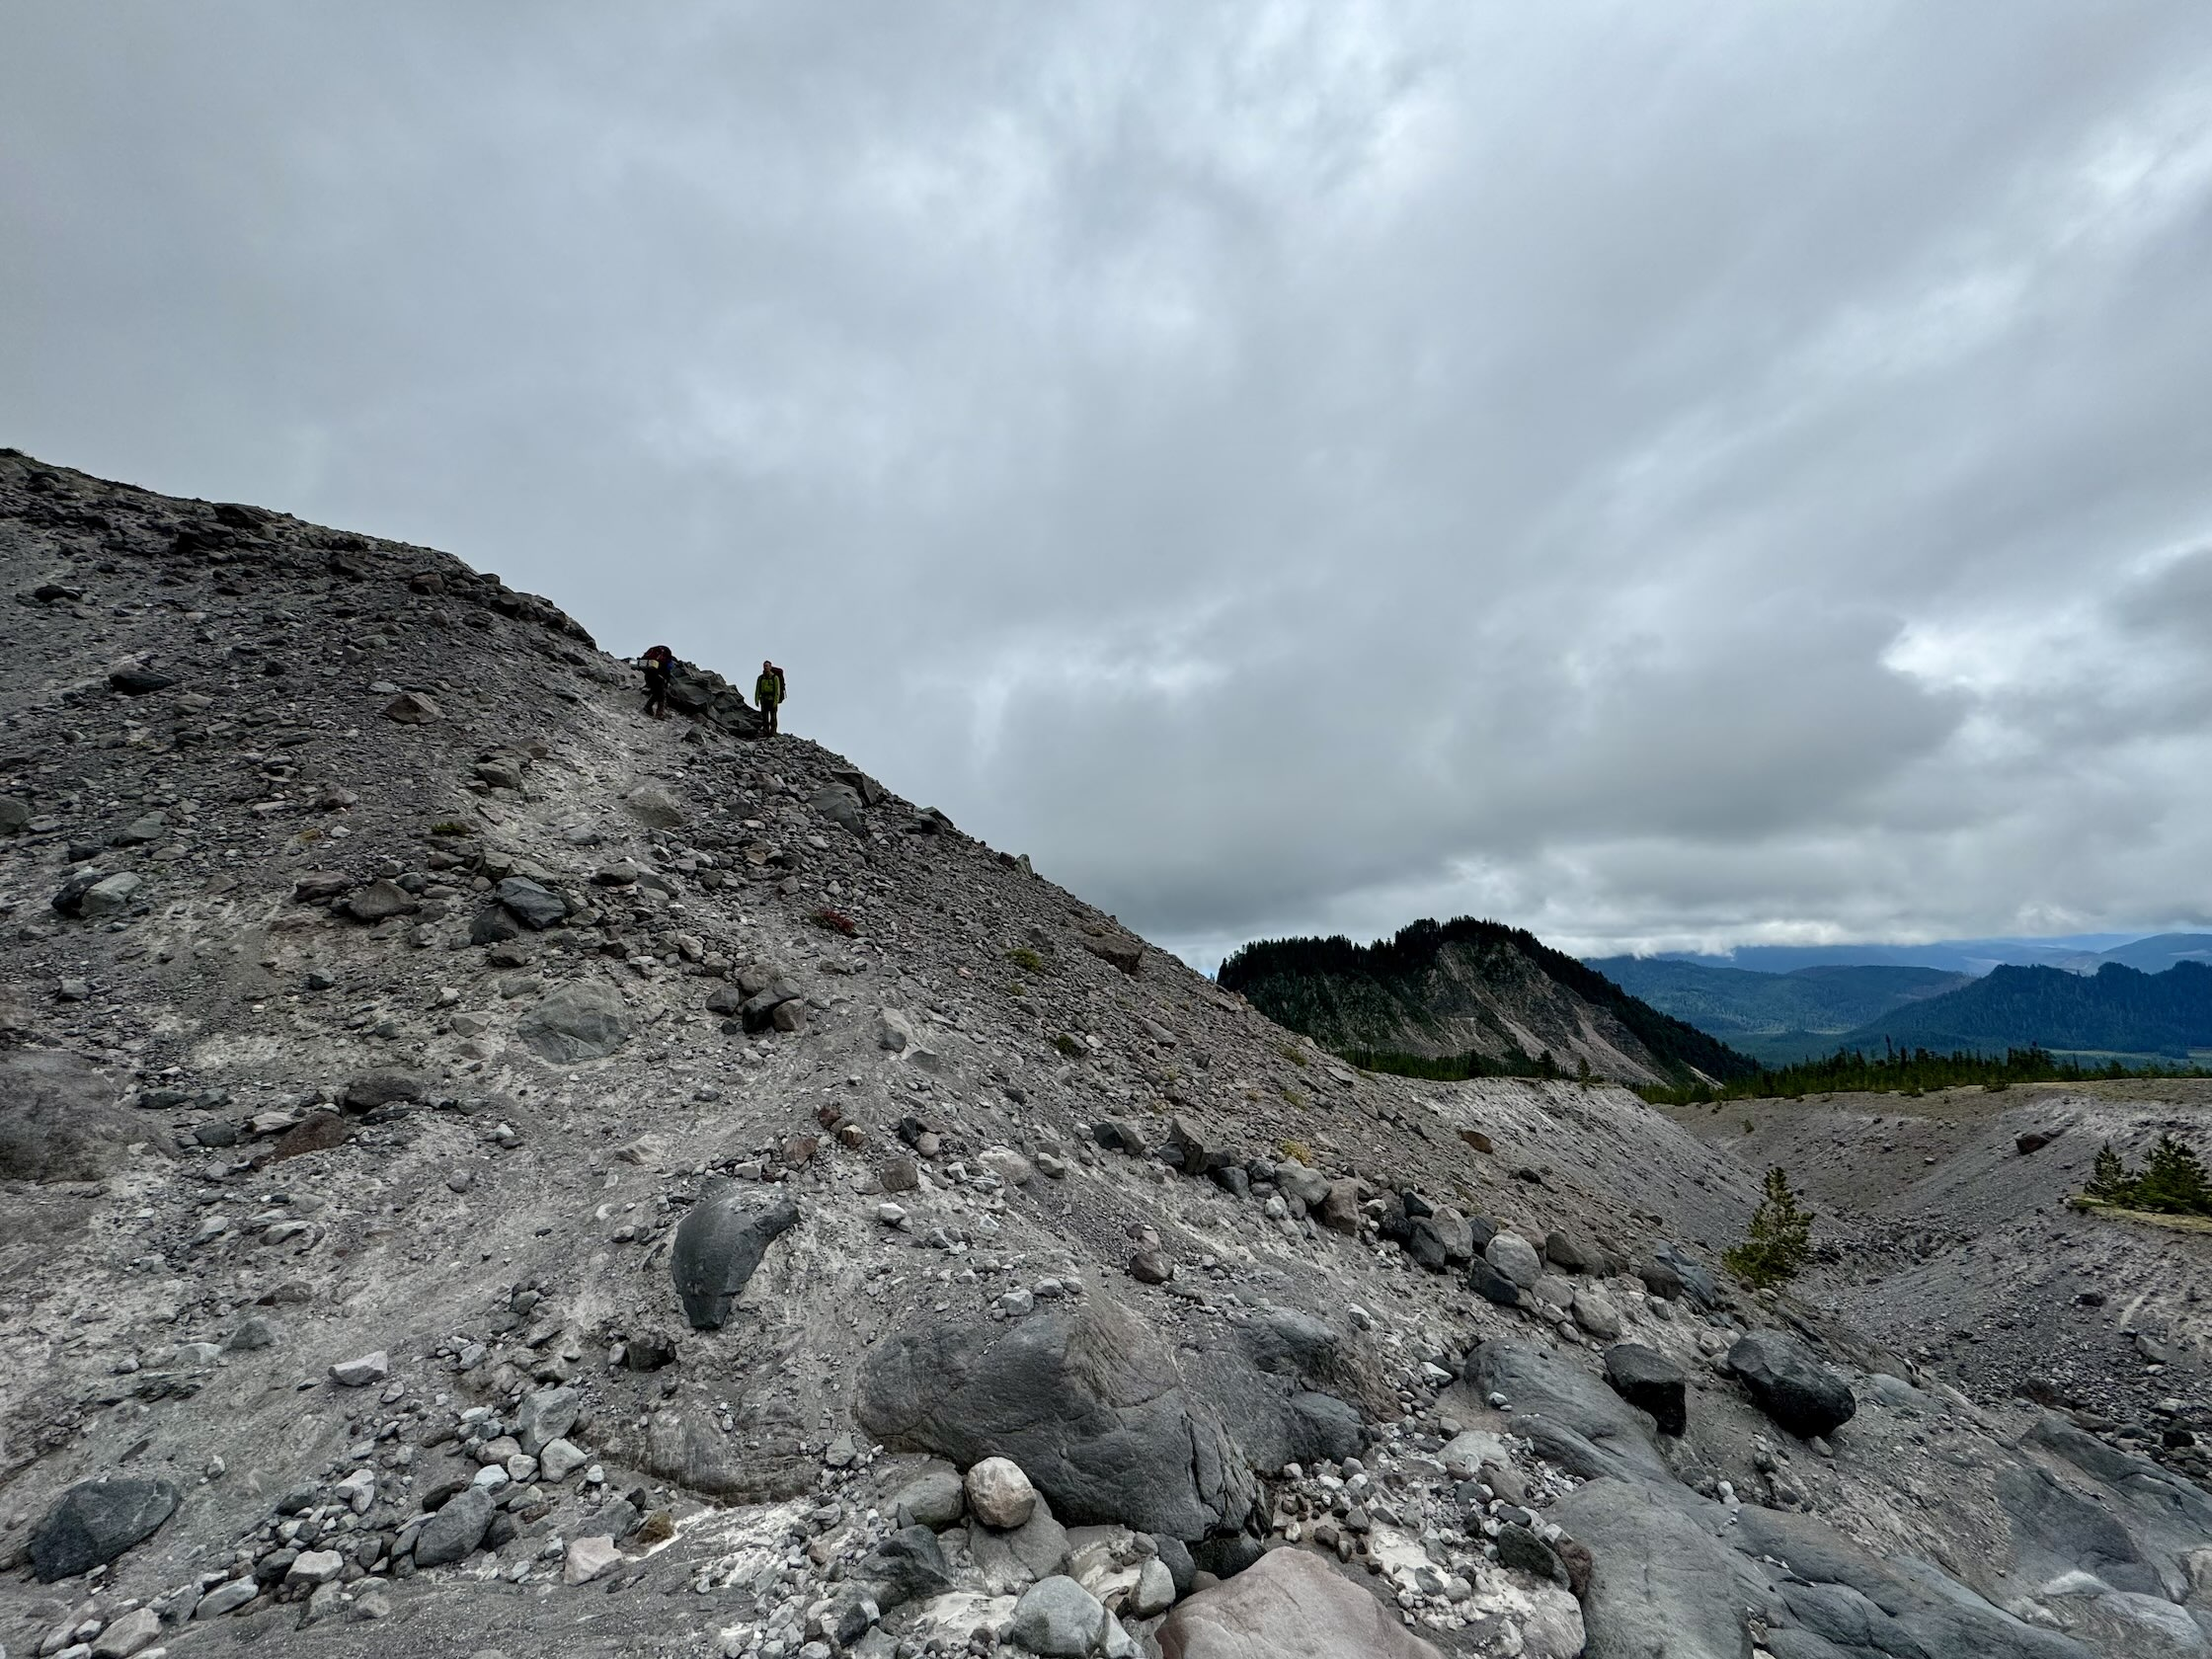
\includegraphics[width=\paperwidth,height=\paperheight]{..//photos/IMG_3031.jpg}} 
\begin{frame}
\begin{center}
\vspace{28ex}
{\color{white} {\huge If time allows...}}
\\
\vspace{3ex}
{\color{white} {\Large My possible project is understanding growth responses to climate and provenance}}

\end{center}
\end{frame}
}

	\frame{
		\frametitle{How does provenance and climate affect tree height?}
			\begin{itemize}
			\item I'd like to build a model that could predict tree height for one species based on where the tree is planted and the provenance of the tree
			\item I think trees grow bigger where it's warmer (and I will start by imagining that temperature is the only important thing on earth)
			\item But I also think there's local adaptation ... 
			\end{itemize}
	}
	
	
	\frame{
		\frametitle{How does provenance and climate affect tree height?}
		\framesubtitle{Imagine I have data from 17 common gardens x 128 provenances}
		\noindent 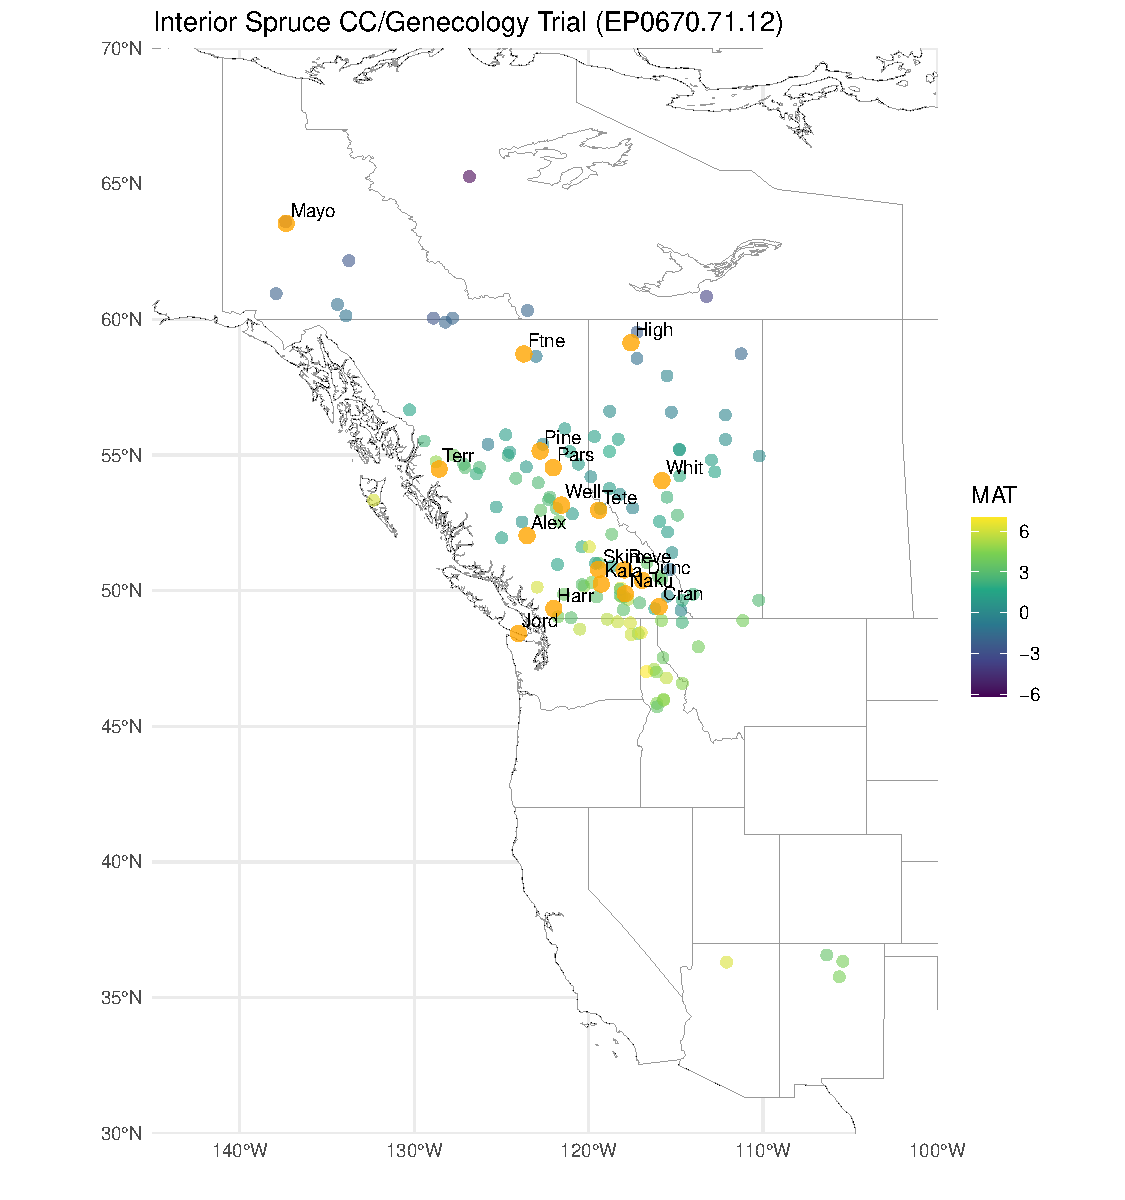
\includegraphics[width=0.6\textwidth]{..//analyses/figures/mapofsites.pdf} 
	}
	
		\frame{
		\frametitle{How does provenance and climate affect tree height?}
		\framesubtitle{I am still on the stage of thinking on figures and math ... }
			\begin{itemize}
			\item I could pretend that provenance is just adding some height up or down and trees grow linearly with temperature ... 
			\begin{align*}
			\hat{y} & = \alpha_0 + \alpha_{provenance} + \beta (C) \\
			\alpha_{provenance} & \sim MVN(0, \sigma_{\alpha}^2)\\
			y & \sim normal(\hat{y}, \sigma_y^2)\\
			\end{align*}
			... which seems wrong
			\end{itemize}
	}



\end{document}